\documentclass[11pt,a4paper]{article}
\usepackage[margin=2.3cm]{geometry}
\usepackage{graphicx,booktabs,amsmath,hyperref,caption,array}
\usepackage[T1]{fontenc}\usepackage{lmodern}
\hypersetup{colorlinks=true,linkcolor=black,urlcolor=blue}
\setlength{\parskip}{0.5em}\setlength{\parindent}{0pt}
\title{Reproducing the Index Selection Evaluation on TPC-H (SF10):\\ Results and Comparison with Kossmann et al.}
\author{Databases course project -- interim report}
\date{21 November 2026}
\begin{document}
\maketitle

\begin{abstract}
We re-ran the TPC-H scale-factor-10 experiment of Kossmann et al.\ (\emph{``Magic Mirror in My Hand, Which Is the Best in the Land?''}, PVLDB 13(11), 2020) on a current software stack (PostgreSQL 18.7, HypoPG 1.4.5) using the authors' evaluation platform. All eight algorithms were run over 112 parameter points with three repetitions each. The qualitative picture of the paper is reproduced: the same cost cliff, the same cluster of well-performing algorithms and the same ranking of run times. We also observe three differences that we report rather than hide: the cliff sits at a smaller budget, CoPhy ends up about 4 points better than in the paper's figure, and absolute run times are 2--10$\times$ lower.
\end{abstract}

\section{Setup}
\textbf{Workload.} TPC-H, scale factor 10, 19 queries (queries 2, 17 and 20 excluded, as in the paper). \textbf{Metric.} Relative workload cost: the optimizer-estimated cost of the workload under the selected indexes divided by its cost without indexes (lower is better), obtained with what-if (hypothetical) indexes. \textbf{Algorithms.} Extend, Relaxation, DTA Anytime, CoPhy, DB2Advis, AutoAdmin, Drop and Dexter. Storage-budget algorithms ran at 16 budgets from 250 to 15\,000\,MB; AutoAdmin and Drop at 1--13 indexes; Dexter at 5 thresholds. All other settings follow the repository configuration \texttt{tpch\_sf10\_paper.json}. Every point was run three times.

\begin{table}[h]\centering\small
\begin{tabular}{lll}\toprule
 & Paper & This reproduction\\\midrule
DBMS & PostgreSQL 12.1 & PostgreSQL 18.7\\
HypoPG & commit 238cca5 & 1.4.5\\
Dexter & -- & 0.6.3\\
CoPhy solver & Gurobi (AMPL) & Gurobi 13 via PuLP 3 (in-platform)\\
CoPhy index width & 2 & 3 (main run); 2 (re-run, Sec.~\ref{sec:cophy})\\
Repetitions & -- & 3\\\bottomrule
\end{tabular}
\caption{Differences between the paper's setup and ours. Hardware is also different.}
\end{table}

\section{Results}
Figure~\ref{fig:main} shows solution quality and run time over index storage consumption; Table~\ref{tab:quality} gives selected points.

\begin{figure}[h]\centering
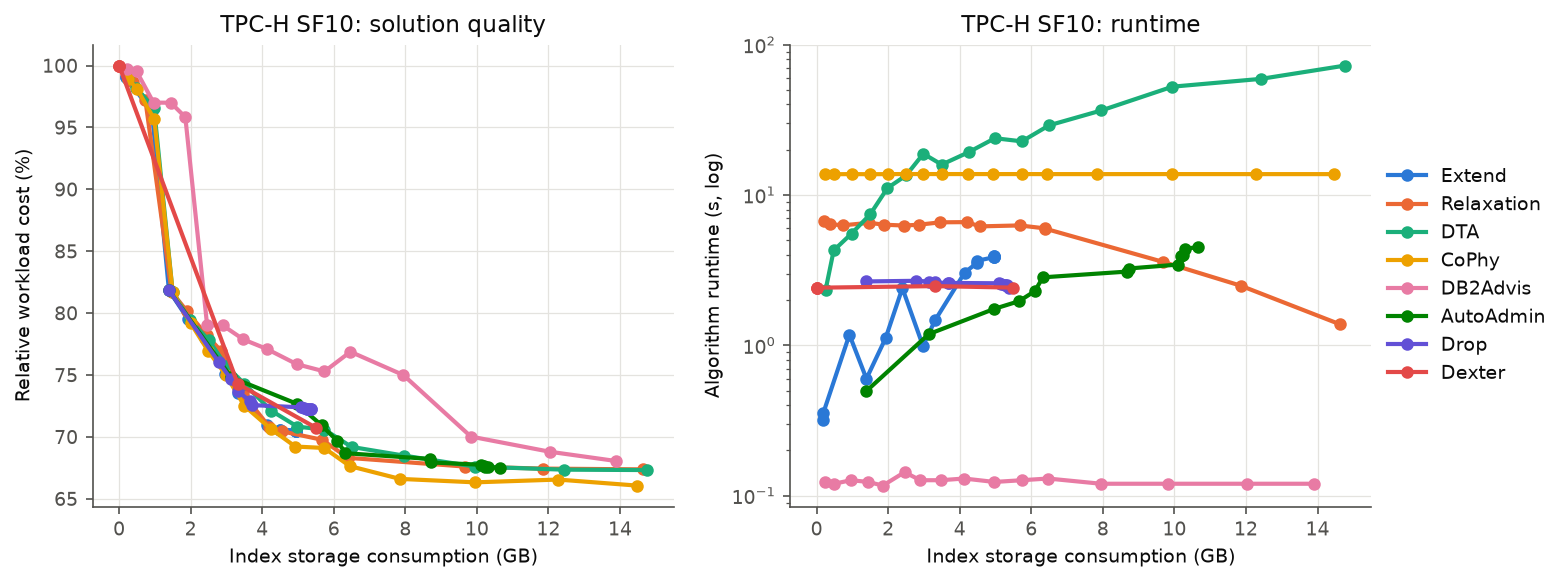
\includegraphics[width=\textwidth]{tpch_sf10_reproduction.png}
\caption{TPC-H SF10: relative workload cost (left) and algorithm run time (right, log scale), mean of three repetitions.}\label{fig:main}
\end{figure}

\begin{table}[h]\centering\small
\begin{tabular}{lrrrrrrr}\toprule
Budget (MB) & 1000 & 1500 & 3000 & 5000 & 8000 & 10000 & 15000\\\midrule
Extend & 96.3 & 81.8 & 75.1 & 70.6 & 70.5 & 70.5 & 70.5\\
Relaxation & 97.2 & 81.7 & 77.0 & 70.4 & 68.3 & 67.6 & 67.4\\
DTA Anytime & 96.5 & 81.7 & 75.8 & 70.8 & 68.5 & 67.6 & 67.3\\
CoPhy (width 3) & 95.7 & 81.7 & 75.0 & 69.2 & 66.6 & 66.3 & 66.1\\
CoPhy (width 2) & 96.1 & 81.7 & 75.0 & 70.2 & 67.9 & 67.6 & 67.4\\
DB2Advis & 97.0 & 97.0 & 79.0 & 75.9 & 75.0 & 70.0 & 68.0\\\bottomrule
\end{tabular}
\caption{Relative workload cost (\%), mean of three repetitions (CoPhy width 2: three-run mean of the re-run). Extend stops adding indexes at about 5\,GB, so its value stays constant.}\label{tab:quality}
\end{table}

\begin{table}[h]\centering\small
\begin{tabular}{lrrl}\toprule
Algorithm & Best cost (\%) & Run time (s) & Setting\\\midrule
AutoAdmin & 67.5 & 4.5 & 13 indexes\\
Drop & 72.2 & 2.4 & 13 indexes\\
Dexter & 70.7 & 2.4 & 10\% threshold (74.3 at 50\%)\\\bottomrule
\end{tabular}
\caption{Algorithms parameterized by index count or threshold rather than storage.}
\end{table}

\textbf{Observations.}
(i)~All storage-budget algorithms except DB2Advis follow almost the same curve. Below about 1.4\,GB (budget 1000\,MB) nothing helps; once the budget admits a single large index on \texttt{lineitem.l\_orderkey}, cost drops from $\approx$96\% to $\approx$82\% for every algorithm at the same budget. A second, smaller drop follows by 2.5--3\,GB.
(ii)~Beyond about 6\,GB, Relaxation, DTA, AutoAdmin and CoPhy end within 67.3--67.7\% (CoPhy at width 2), i.e.\ within the repetition spread; Extend stops at 70.5\%.
(iii)~DB2Advis is fast (0.1\,s) but needs more space for the same quality: its cost stays at 79--75\% until 8\,GB.
(iv)~Drop is the weakest of the index-count algorithms; AutoAdmin matches the leaders with 13 indexes.
(v)~Run time separates the algorithms by orders of magnitude: DB2Advis $\approx$0.1\,s, Extend 0.3--3.9\,s, Dexter and Drop $\approx$2.5\,s, AutoAdmin 0.5--4.5\,s, Relaxation 1.4--6.7\,s, CoPhy 13.8\,s (flat, dominated by what-if calls), DTA rising from 2\,s to 73\,s with the budget. Figure~\ref{fig:calls} shows quality against what-if calls: Extend and AutoAdmin reach good quality with the fewest calls, DTA needs the most among the iterative algorithms, and CoPhy always issues $\approx$23\,000 calls.

\begin{figure}[h]\centering
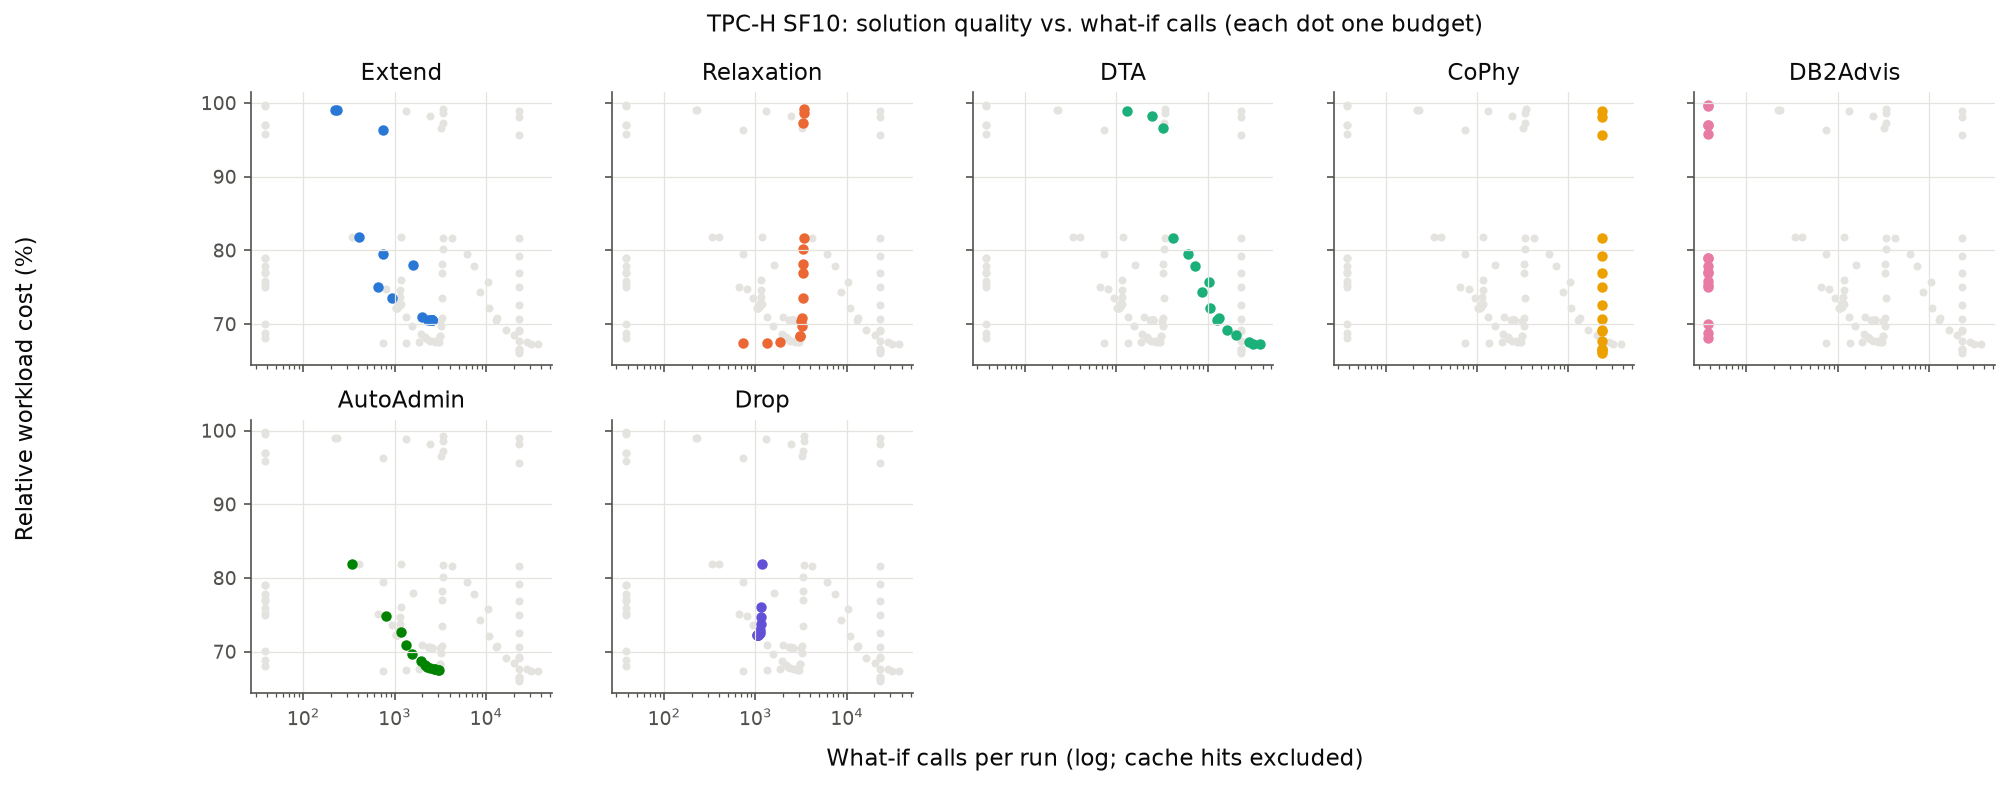
\includegraphics[width=\textwidth]{tpch_sf10_quality_vs_calls.png}
\caption{Solution quality versus what-if calls per run (log scale; cache hits excluded); each dot is one budget.}\label{fig:calls}
\end{figure}

\section{Comparison with the paper}
We compared against Figure~3(a) and (d) of the paper. Paper values are read off the plots and are accurate to about $\pm$1--2 percentage points or seconds; the conclusions below do not depend on this.

\begin{table}[h]\centering\small
\begin{tabular}{p{4.0cm}p{4.9cm}p{5.2cm}}\toprule
 & Paper (Fig.~3a/d) & Ours\\\midrule
Cost cliff & at $\approx$2\,GB, $\approx$94\% $\to$ $\approx$80\% & at $\approx$1.4\,GB, $\approx$96\% $\to$ $\approx$82\%\\
Quality near 10\,GB & $\approx$68--70\%; Relaxation lowest & 66.3--70.7\%; CoPhy lowest; Relaxation, DTA, AutoAdmin 67.6--67.7\%\\
CoPhy quality & $\approx$72\% at 6.5--8.7\,GB, not among the best & 69.1\% at 5.75\,GB, 66.6\% at 8\,GB (width 3); 67.9\% at 8\,GB (width 2)\\
DB2Advis & $\approx$75\% plateau to $\approx$8\,GB & 75--77\% to 8\,GB, 70\% at 10\,GB\\
Dexter & $\approx$71\% at $\approx$5.5\,GB & 70.7\% at $\approx$5.4\,GB\\
DTA run time (10\,GB) & jagged, 100--137\,s & smooth, 52\,s\\
CoPhy run time & flat, $\approx$150\,s & flat, 13.8\,s\\
Drop run time & flat, $\approx$16\,s & flat, 2.5\,s\\
DB2Advis run time & $\approx$0 & 0.1\,s\\\bottomrule
\end{tabular}
\caption{Paper versus reproduction.}
\end{table}

\textbf{What reproduces.} The shape of every curve, the cliff and the cluster of near-equal algorithms, DB2Advis being fast but space-hungry, Dexter's operating point, and the ordering of run times (DB2Advis $\ll$ Extend/Drop/Dexter $<$ Relaxation $<$ CoPhy, with DTA growing with budget).

\textbf{What differs.}
\begin{enumerate}
\item \emph{Cliff position.} The large index becomes affordable at about 1.4\,GB instead of 2\,GB. In our results the selection that includes \texttt{lineitem.l\_orderkey} fits a 1500\,MB budget (1498\,MB estimated total for four indexes), so HypoPG's size estimate for that index is clearly below the paper's. Plausible causes are the PostgreSQL version (e.g.\ btree deduplication) and the newer HypoPG estimator; we have not yet isolated one. A direct comparison of the estimated and real size of that index is planned.
\item \emph{CoPhy quality.} The paper's CoPhy is not among the best; ours is. Our main run used index width 3 for CoPhy while the paper states width 2. The re-run at width 2 (Sec.~\ref{sec:cophy}) removes only about 1 point, so index width explains the gap only in small part. About 4 points remain unexplained; the solver and PostgreSQL versions are candidates.
\item \emph{Absolute run times} are 2--10$\times$ lower than in the paper with the same shapes. We attribute this to newer hardware, PostgreSQL and solver versions, but did not isolate it. We therefore compare orderings and trends, not seconds.
\end{enumerate}
Differences (2) and (3) concern the platform's own numbers and not the algorithms' rank order at small and medium budgets, where all curves agree with the paper.

\section{CoPhy index-width check}\label{sec:cophy}
To test whether the CoPhy discrepancy comes from the index width, we re-ran only CoPhy (and the no-index baseline) with width 2, three repetitions, same budgets. Quality changed from 69.1 to 69.8\% at 5.75\,GB, from 66.6 to 67.9\% at 8\,GB and from 66.3 to 67.6\% at 10\,GB (Table~\ref{tab:quality}). The three repetitions differ by at most 0.2 points, making CoPhy the most stable algorithm in our runs. CoPhy's final quality (67.4\%) now equals that of Relaxation, DTA and AutoAdmin, whereas the paper shows it clearly worse.

\section{Run-to-run variability}
PostgreSQL's \texttt{ANALYZE} samples rows randomly, so identical re-runs see slightly different statistics (for example, the estimated number of distinct \texttt{lineitem.l\_orderkey} values was 430\,030, 417\,382 and 410\,520 in the three CoPhy re-run repetitions). The maximum spread over repetitions across all parameter points is 3.15 points for DTA, 2.51 for CoPhy (width 3), 1.70 for Relaxation, 1.57 for DB2Advis, 1.09 for AutoAdmin, 1.07 for Extend, 0.39 for Drop and 0.29 for Dexter. Differences of one to two points between Relaxation, DTA, AutoAdmin and CoPhy at large budgets are therefore within noise with $n=3$; we do not claim a ranking among them.

\section{Limitations}
Three repetitions are too few for confidence intervals. The paper's values were read from figures. Only the TPC-H workload at SF10 has been reproduced so far; TPC-DS and JOB are open. Costs are optimizer estimates from hypothetical indexes, as in the paper, and were not validated by executing the queries.

\section{Conclusion and next steps}
The central findings of the original TPC-H evaluation hold on PostgreSQL 18: index selection quality is determined mainly by whether a few key indexes fit, most algorithms converge to the same cost, and the algorithms differ chiefly in run time and in how many what-if calls they need. We will (a) determine the cause of the shifted cliff by comparing HypoPG's size estimate with real index sizes, (b) extend the reproduction to TPC-DS and JOB, and (c) add budget-aware algorithms (Wii, Esc) and compare them with the original eight under a what-if-call budget.

\section*{Reproducibility}
Repository: \texttt{RameezWahid/magic-mirror-revisited}, branch \texttt{sf10-arijit}; commit of the platform \texttt{8e8a33f}. Results: \texttt{benchmark\_results/tpch\_sf10\_paper\_pg18.7} (3 repetitions), \texttt{tpch\_sf10\_cophy\_w2\_pg18.7} (CoPhy width 2), analysis in \texttt{benchmark\_results/sf10\_analysis}. Environment: PostgreSQL 18.7, HypoPG 1.4.5, Dexter 0.6.3, gurobipy 13.x, PuLP 3.x (PuLP 4 is incompatible with the CoPhy code).

\section*{References}
\begin{enumerate}\small
\item J.\ Kossmann, S.\ Halfpap, M.\ Jankrift, R.\ Schlosser. Magic Mirror in My Hand, Which Is the Best in the Land? An Experimental Evaluation of Index Selection Algorithms. PVLDB 13(11), 2020.
\item S.\ Halfpap et al. Looking Deeply into the Magic Mirror. PVLDB 17, 2024 (demonstration; platform used here).
\end{enumerate}
\end{document}
